\documentclass[11pt]{article}
\usepackage{graphicx}
\usepackage{float}
\usepackage{amsmath}
\usepackage[margin=1.25in]{geometry}
\title{ECE 5746 Lab 2}
\author{Abiola Bolaji}
\date{}
\begin{document}
\maketitle

\section*{1\quad RTL Design and Verification}

\textbf{Design.} The multiplier (\texttt{mul.sv}, module \texttt{mult}) takes two 16-bit unsigned inputs \texttt{inp\_a} and \texttt{inp\_b} and registers their 32-bit product: on each rising edge of \texttt{clk}, \texttt{prod <= inp\_a * inp\_b}. An asynchronous, active-high \texttt{rst} clears \texttt{prod} to 0. The product is 32 bits wide, so the largest result ($\texttt{0xFFFF} \times \texttt{0xFFFF}$) fits without overflow. Because the output is registered, synthesis times the path from the input ports through the multiplier logic to the \texttt{prod} flip-flops, which is the critical path reported in \texttt{syn\_timing.rpt}.

\textbf{Testbench.} \texttt{tb\_mul.sv} generates a 10\,ns clock, holds \texttt{rst} high for the first 10\,ns, and applies 5 input pairs, each held for 20\,ns (2 clock cycles). The vectors cover small values, zero, the largest inputs (which exercise every partial-product bit and the top bits of \texttt{prod}), and a mixed value. The testbench waits one extra 20\,ns after the last vector before \texttt{\$finish}, so the last product is visible in the waveform. I checked each product in the QuestaSim waveform against the expected value in Table~\ref{tab:rtl}.

\begin{table}[H]
\begin{center}
\small
\begin{tabular}{r|c|c|c|r|r}
\hline
applied (ns) & inp\_a & inp\_b & expected prod & decimal & prod updates (ns) \\
\hline
0 & \texttt{0001} & \texttt{0002} & \texttt{00000002} & 2 & 15 \\
20 & \texttt{0003} & \texttt{0004} & \texttt{0000000c} & 12 & 25 \\
40 & \texttt{0000} & \texttt{0000} & \texttt{00000000} & 0 & 45 \\
60 & \texttt{ffff} & \texttt{ffff} & \texttt{fffe0001} & 4{,}294{,}836{,}225 & 65 \\
80 & \texttt{00c0} & \texttt{0acf} & \texttt{00081b40} & 531{,}264 & 85 \\
\hline
\end{tabular}
\end{center}
\caption{Test vectors from \texttt{tb\_mul.sv}. Expected products are computed from the inputs; the waveform in Figure~\ref{fig:rtl} shows the same values on \texttt{prod}.}
\label{tab:rtl}
\end{table}
\begin{figure}[H]
\centering
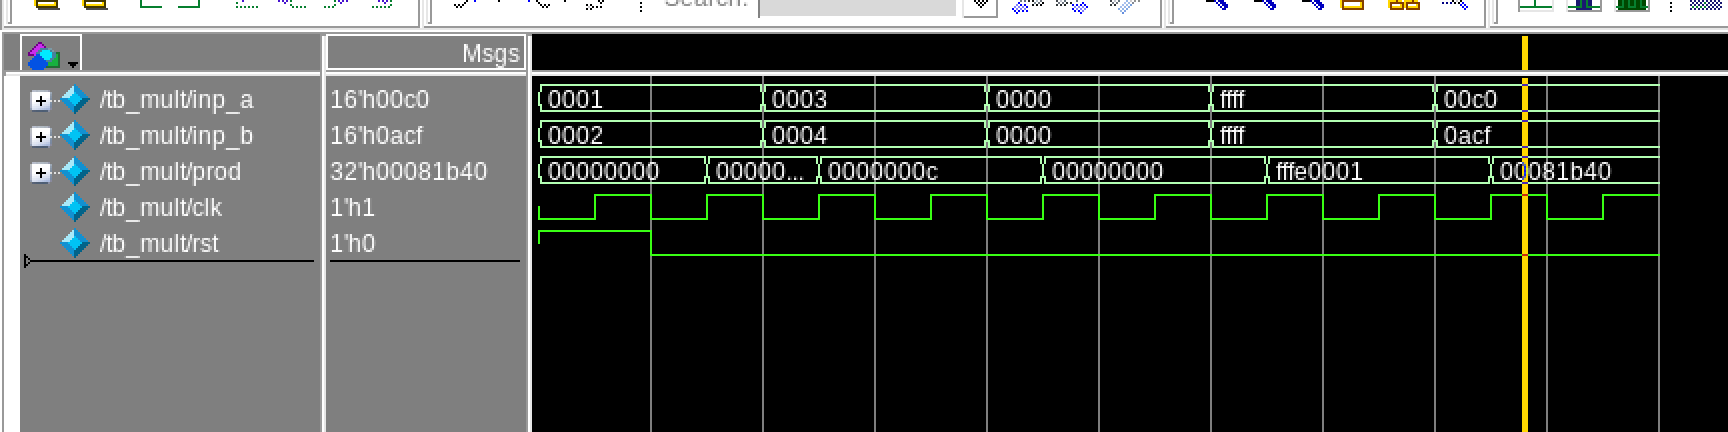
\includegraphics[width=\textwidth]{figures/rtl_waveform.png}
\caption{QuestaSim waveform of \texttt{tb\_mult}: inputs, registered product, clock and reset.}
\label{fig:rtl}
\end{figure}
\textbf{Result.} All 5 products match the expected values. While \texttt{rst} is high, \texttt{prod} stays at 0, so the first product appears at 15\,ns, on the first rising edge after reset is released. After that, each new product appears on the first rising edge after the inputs change, which is the one-register latency of the design. $\texttt{0xFFFF} \times \texttt{0xFFFF} = \texttt{0xFFFE0001}$ confirms the full 32-bit result is kept.

\section*{2\quad SVT20: Fmax and Energy Sweep}

For the standard-$V_t$ cells (BWP20P90), I swept the clock period in \texttt{lab2.sh} and checked the worst slack in \texttt{syn\_timing.rpt}. I use $clk\_period_{min} = 0.33$\,ns (chosen at 0.01\,ns precision; a finer search showed 0.327\,ns also meets timing), so $F_{max} = 1/0.33\,\text{ns} = 3030$\,MHz. I then synthesized the design at $1\times$ to $1000\times$ this clock period.

Energy per cycle is computed from \texttt{syn\_power.rpt}: $P_{Dyn}$ is switching plus internal power (mW), $P_{Leak}$ is leakage power (reported in nW), and $E_{Dyn} = P_{Dyn} \times clk\_period$, $E_{Leak} = P_{Leak} \times clk\_period$, $E_{total} = E_{Dyn} + E_{Leak}$. With mW and ns, the energies are in pJ.
\begin{center}
\small
\begin{tabular}{r|r|r|r|r|r|r|r}
\hline
$\times$ min & clk (ns) & f (MHz) & slack (ns) & area ($\mu m^2$) & $E_{Dyn}$ (pJ) & $E_{Leak}$ (pJ) & $E_{total}$ (pJ) \\
\hline
1.00 & 0.33 & 3030.3 & 0.00 & 525.7 & 0.9227 & 3.53e-04 & 0.9230 \\
1.05 & 0.3465 & 2886.0 & 0.00 & 440.0 & 0.7540 & 2.69e-04 & 0.7543 \\
1.10 & 0.363 & 2754.8 & 0.00 & 407.6 & 0.6951 & 2.45e-04 & 0.6954 \\
1.15 & 0.3795 & 2635.0 & 0.00 & 380.5 & 0.6391 & 2.21e-04 & 0.6393 \\
1.20 & 0.396 & 2525.3 & 0.00 & 371.8 & 0.6292 & 2.20e-04 & 0.6295 \\
1.25 & 0.4125 & 2424.2 & 0.00 & 365.6 & 0.6150 & 2.20e-04 & 0.6153 \\
1.30 & 0.429 & 2331.0 & 0.00 & 359.5 & 0.6045 & 2.26e-04 & 0.6047 \\
1.40 & 0.462 & 2164.5 & 0.00 & 355.5 & 0.5983 & 2.41e-04 & 0.5985 \\
1.50 & 0.495 & 2020.2 & 0.00 & 356.1 & 0.6014 & 2.59e-04 & 0.6017 \\
1.75 & 0.5775 & 1731.6 & 0.00 & 352.1 & 0.5983 & 2.99e-04 & 0.5986 \\
2.00 & 0.66 & 1515.2 & 0.00 & 348.2 & 0.5881 & 3.37e-04 & 0.5884 \\
3.00 & 0.99 & 1010.1 & 0.00 & 327.4 & 0.5693 & 3.99e-04 & 0.5696 \\
5.00 & 1.65 & 606.1 & 0.51 & 318.0 & 0.5231 & 6.07e-04 & 0.5237 \\
10.00 & 3.3 & 303.0 & 2.16 & 318.2 & 0.5214 & 1.19e-03 & 0.5226 \\
100.00 & 33 & 30.3 & 31.86 & 318.2 & 0.5214 & 1.19e-02 & 0.5333 \\
1000.00 & 330 & 3.0 & 328.87 & 318.2 & 0.5214 & 1.19e-01 & 0.6404 \\
\hline
\end{tabular}
\end{center}
\begin{figure}[H]
\centering
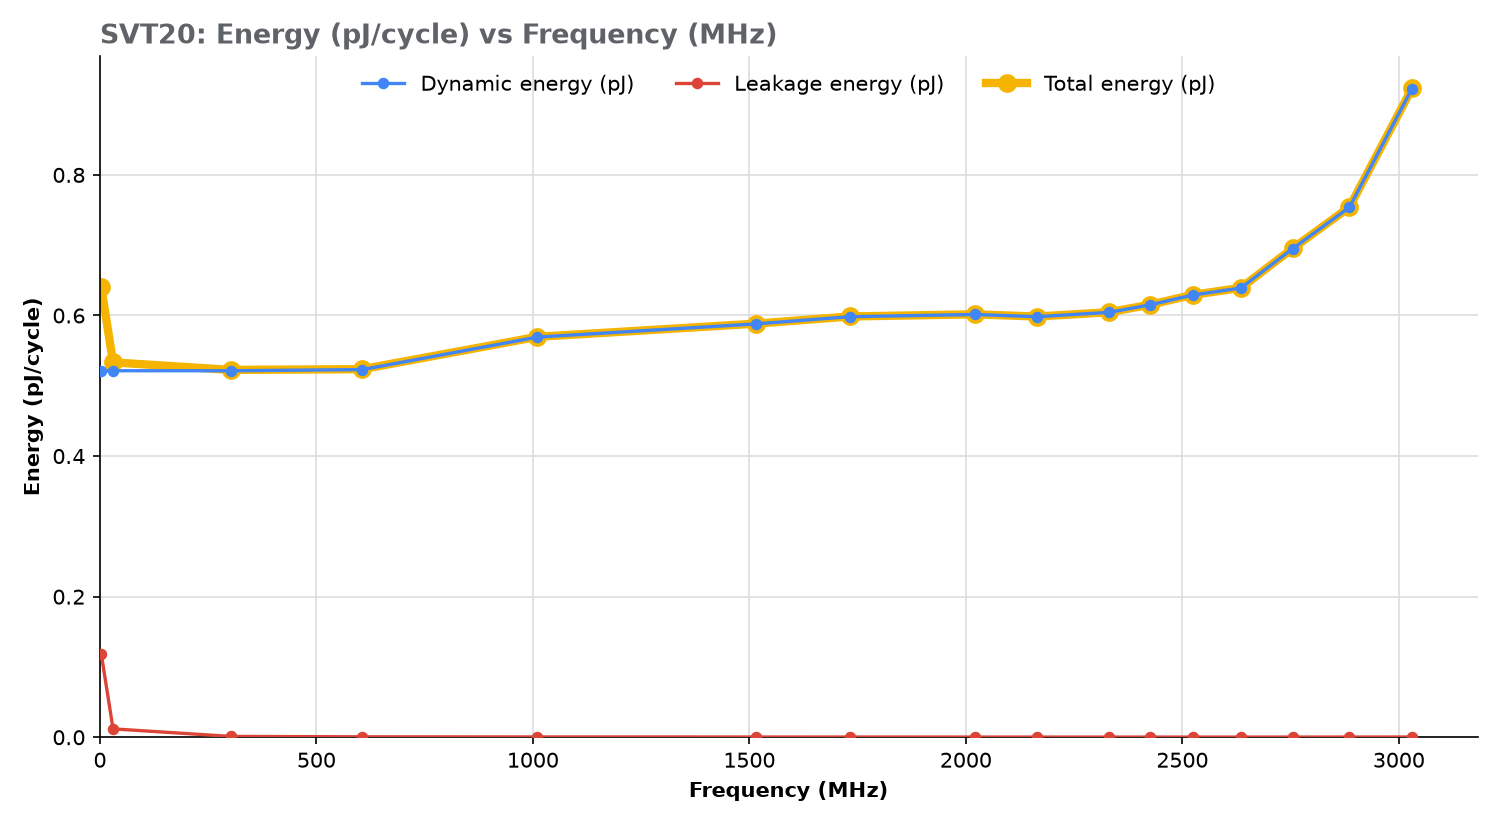
\includegraphics[width=0.95\textwidth]{figures/energy_SVT20.png}
\caption{SVT20: dynamic, leakage and total energy per cycle vs frequency. Each marker is one synthesis run.}
\label{fig:energy_SVT20}
\end{figure}
The minimum total energy is 0.5226\,pJ/cycle at 303\,MHz (3.3\,ns, $10\times$). At $F_{max}$ it is 0.9230\,pJ/cycle.

\section*{3\quad LVT20: Fmax and Energy Sweep}

For the low-$V_t$ cells (BWP20P90LVT), I swept the clock period in \texttt{lab2.sh} and checked the worst slack in \texttt{syn\_timing.rpt}. I use $clk\_period_{min} = 0.244$\,ns (0.244\,ns meets timing and 0.242\,ns does not), so $F_{max} = 1/0.244\,\text{ns} = 4098$\,MHz. I then synthesized the design at $1\times$ to $1000\times$ this clock period.

Energy per cycle is computed from \texttt{syn\_power.rpt}: $P_{Dyn}$ is switching plus internal power (mW), $P_{Leak}$ is leakage power (reported in nW), and $E_{Dyn} = P_{Dyn} \times clk\_period$, $E_{Leak} = P_{Leak} \times clk\_period$, $E_{total} = E_{Dyn} + E_{Leak}$. With mW and ns, the energies are in pJ.
\begin{center}
\small
\begin{tabular}{r|r|r|r|r|r|r|r}
\hline
$\times$ min & clk (ns) & f (MHz) & slack (ns) & area ($\mu m^2$) & $E_{Dyn}$ (pJ) & $E_{Leak}$ (pJ) & $E_{total}$ (pJ) \\
\hline
1.00 & 0.244 & 4098.4 & 0.00 & 525.2 & 0.9894 & 3.27e-03 & 0.9927 \\
1.05 & 0.2562 & 3903.2 & 0.00 & 462.8 & 0.8306 & 2.77e-03 & 0.8334 \\
1.10 & 0.2684 & 3725.8 & 0.00 & 412.7 & 0.7378 & 2.32e-03 & 0.7401 \\
1.15 & 0.2806 & 3563.8 & 0.00 & 391.2 & 0.7158 & 2.17e-03 & 0.7180 \\
1.20 & 0.2928 & 3415.3 & 0.00 & 377.7 & 0.6960 & 2.11e-03 & 0.6981 \\
1.25 & 0.305 & 3278.7 & 0.00 & 367.7 & 0.6771 & 2.06e-03 & 0.6792 \\
1.30 & 0.3172 & 3152.6 & 0.00 & 364.4 & 0.6690 & 2.09e-03 & 0.6711 \\
1.40 & 0.3416 & 2927.4 & 0.00 & 354.8 & 0.6497 & 2.19e-03 & 0.6519 \\
1.50 & 0.366 & 2732.2 & 0.00 & 355.5 & 0.6533 & 2.38e-03 & 0.6557 \\
1.75 & 0.427 & 2341.9 & 0.00 & 352.6 & 0.6448 & 2.75e-03 & 0.6475 \\
2.00 & 0.488 & 2049.2 & 0.00 & 346.9 & 0.6359 & 3.07e-03 & 0.6389 \\
3.00 & 0.732 & 1366.1 & 0.00 & 320.1 & 0.6273 & 3.85e-03 & 0.6312 \\
5.00 & 1.22 & 819.7 & 0.38 & 310.5 & 0.5649 & 5.78e-03 & 0.5706 \\
10.00 & 2.44 & 409.8 & 1.61 & 310.7 & 0.5585 & 1.14e-02 & 0.5699 \\
100.00 & 24.4 & 41.0 & 23.57 & 310.7 & 0.5583 & 1.14e-01 & 0.6720 \\
1000.00 & 244 & 4.1 & 243.17 & 310.7 & 0.5583 & 1.14e+00 & 1.6953 \\
\hline
\end{tabular}
\end{center}
\begin{figure}[H]
\centering
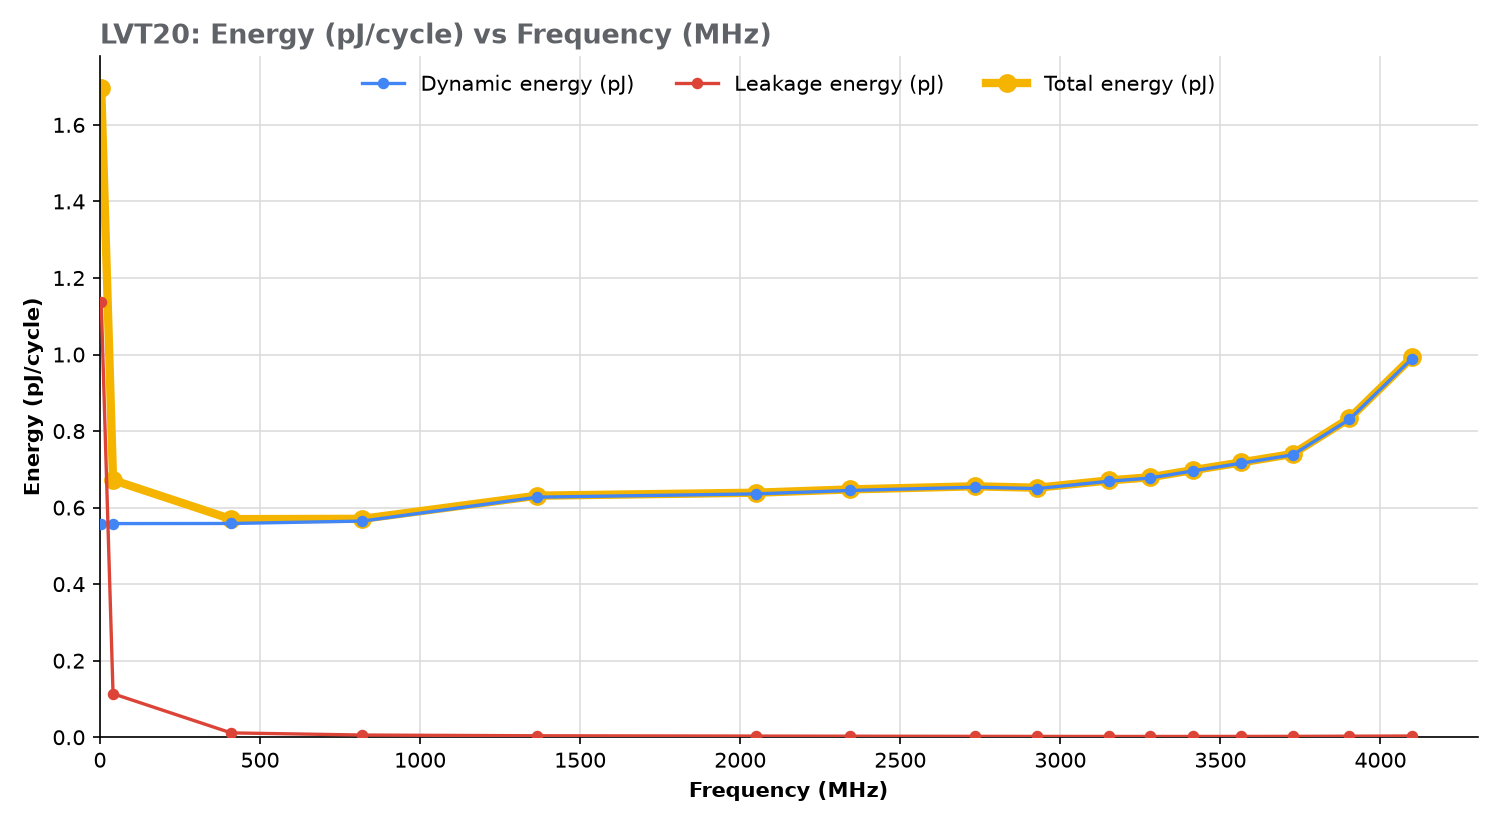
\includegraphics[width=0.95\textwidth]{figures/energy_LVT20.png}
\caption{LVT20: dynamic, leakage and total energy per cycle vs frequency. Each marker is one synthesis run.}
\label{fig:energy_LVT20}
\end{figure}
The minimum total energy is 0.5699\,pJ/cycle at 410\,MHz (2.44\,ns, $10\times$). At $F_{max}$ it is 0.9927\,pJ/cycle.

\section*{4\quad LVT16: Fmax and Energy Sweep}

For the low-$V_t$ cells (BWP16P90LVT), I swept the clock period in \texttt{lab2.sh} and checked the worst slack in \texttt{syn\_timing.rpt}. I use $clk\_period_{min} = 0.22$\,ns (chosen at 0.01\,ns precision: 0.22\,ns meets timing and 0.21\,ns does not), so $F_{max} = 1/0.22\,\text{ns} = 4545$\,MHz. I then synthesized the design at $1\times$ to $1000\times$ this clock period.

Energy per cycle is computed from \texttt{syn\_power.rpt}: $P_{Dyn}$ is switching plus internal power (mW), $P_{Leak}$ is leakage power (reported in nW), and $E_{Dyn} = P_{Dyn} \times clk\_period$, $E_{Leak} = P_{Leak} \times clk\_period$, $E_{total} = E_{Dyn} + E_{Leak}$. With mW and ns, the energies are in pJ.
\begin{center}
\small
\begin{tabular}{r|r|r|r|r|r|r|r}
\hline
$\times$ min & clk (ns) & f (MHz) & slack (ns) & area ($\mu m^2$) & $E_{Dyn}$ (pJ) & $E_{Leak}$ (pJ) & $E_{total}$ (pJ) \\
\hline
1.00 & 0.22 & 4545.5 & 0.00 & 629.8 & 1.2096 & 9.50e-03 & 1.2191 \\
1.05 & 0.231 & 4329.0 & 0.00 & 520.3 & 0.9739 & 7.21e-03 & 0.9811 \\
1.10 & 0.242 & 4132.2 & 0.00 & 434.7 & 0.8027 & 5.30e-03 & 0.8080 \\
1.15 & 0.253 & 3952.6 & 0.00 & 410.8 & 0.7529 & 5.03e-03 & 0.7580 \\
1.20 & 0.264 & 3787.9 & 0.00 & 378.9 & 0.6766 & 4.44e-03 & 0.6811 \\
1.25 & 0.275 & 3636.4 & 0.00 & 370.0 & 0.6639 & 4.32e-03 & 0.6682 \\
1.30 & 0.286 & 3496.5 & 0.00 & 368.8 & 0.6607 & 4.55e-03 & 0.6652 \\
1.40 & 0.308 & 3246.8 & 0.00 & 358.4 & 0.6443 & 4.62e-03 & 0.6490 \\
1.50 & 0.33 & 3030.3 & 0.00 & 359.6 & 0.6491 & 5.15e-03 & 0.6543 \\
1.75 & 0.385 & 2597.4 & 0.00 & 355.9 & 0.6464 & 5.89e-03 & 0.6523 \\
2.00 & 0.44 & 2272.7 & 0.00 & 350.3 & 0.6499 & 6.60e-03 & 0.6565 \\
3.00 & 0.66 & 1515.2 & 0.00 & 319.0 & 0.6178 & 7.85e-03 & 0.6256 \\
5.00 & 1.1 & 909.1 & 0.36 & 310.7 & 0.5544 & 1.18e-02 & 0.5662 \\
10.00 & 2.2 & 454.5 & 1.46 & 310.7 & 0.5544 & 2.35e-02 & 0.5779 \\
100.00 & 22 & 45.5 & 21.26 & 310.7 & 0.5491 & 2.29e-01 & 0.7779 \\
1000.00 & 220 & 4.5 & 219.26 & 310.7 & 0.5467 & 2.29e+00 & 2.8347 \\
\hline
\end{tabular}
\end{center}
\begin{figure}[H]
\centering
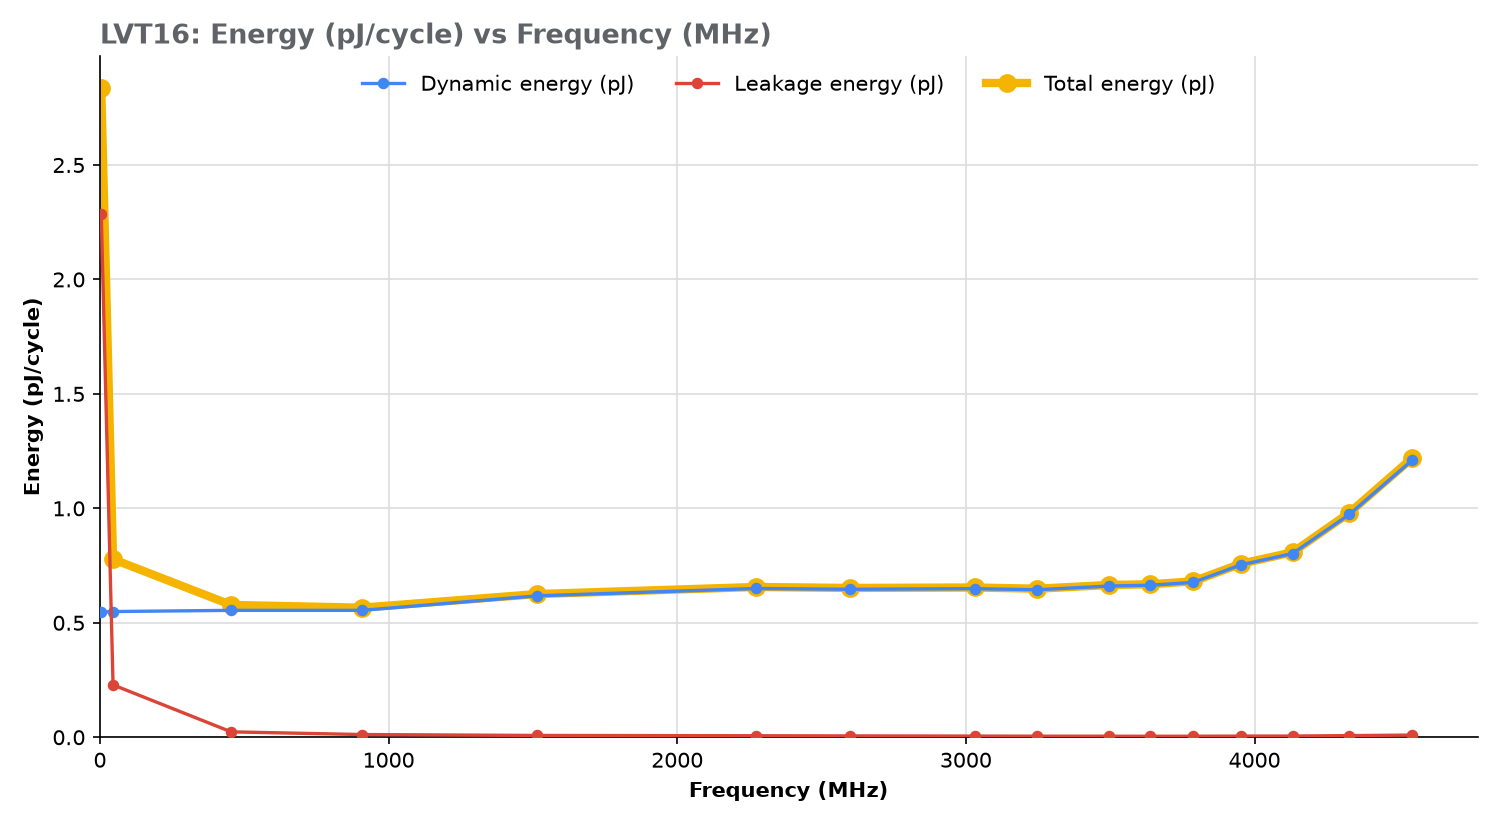
\includegraphics[width=0.95\textwidth]{figures/energy_LVT16.png}
\caption{LVT16: dynamic, leakage and total energy per cycle vs frequency. Each marker is one synthesis run.}
\label{fig:energy_LVT16}
\end{figure}
The minimum total energy is 0.5662\,pJ/cycle at 909\,MHz (1.1\,ns, $5\times$). At $F_{max}$ it is 1.2191\,pJ/cycle.

\section*{5\quad PPA Trends and Optimal Operating Frequency}

Below I discuss the performance, power and area trends for each graph, using \texttt{syn\_area.rpt}, \texttt{syn\_timing.rpt}, \texttt{syn\_power.rpt} and the cell list in \texttt{syn.rpt}. Figure~\ref{fig:ppa} summarizes how the netlist changes with frequency.

\begin{figure}[H]
\centering
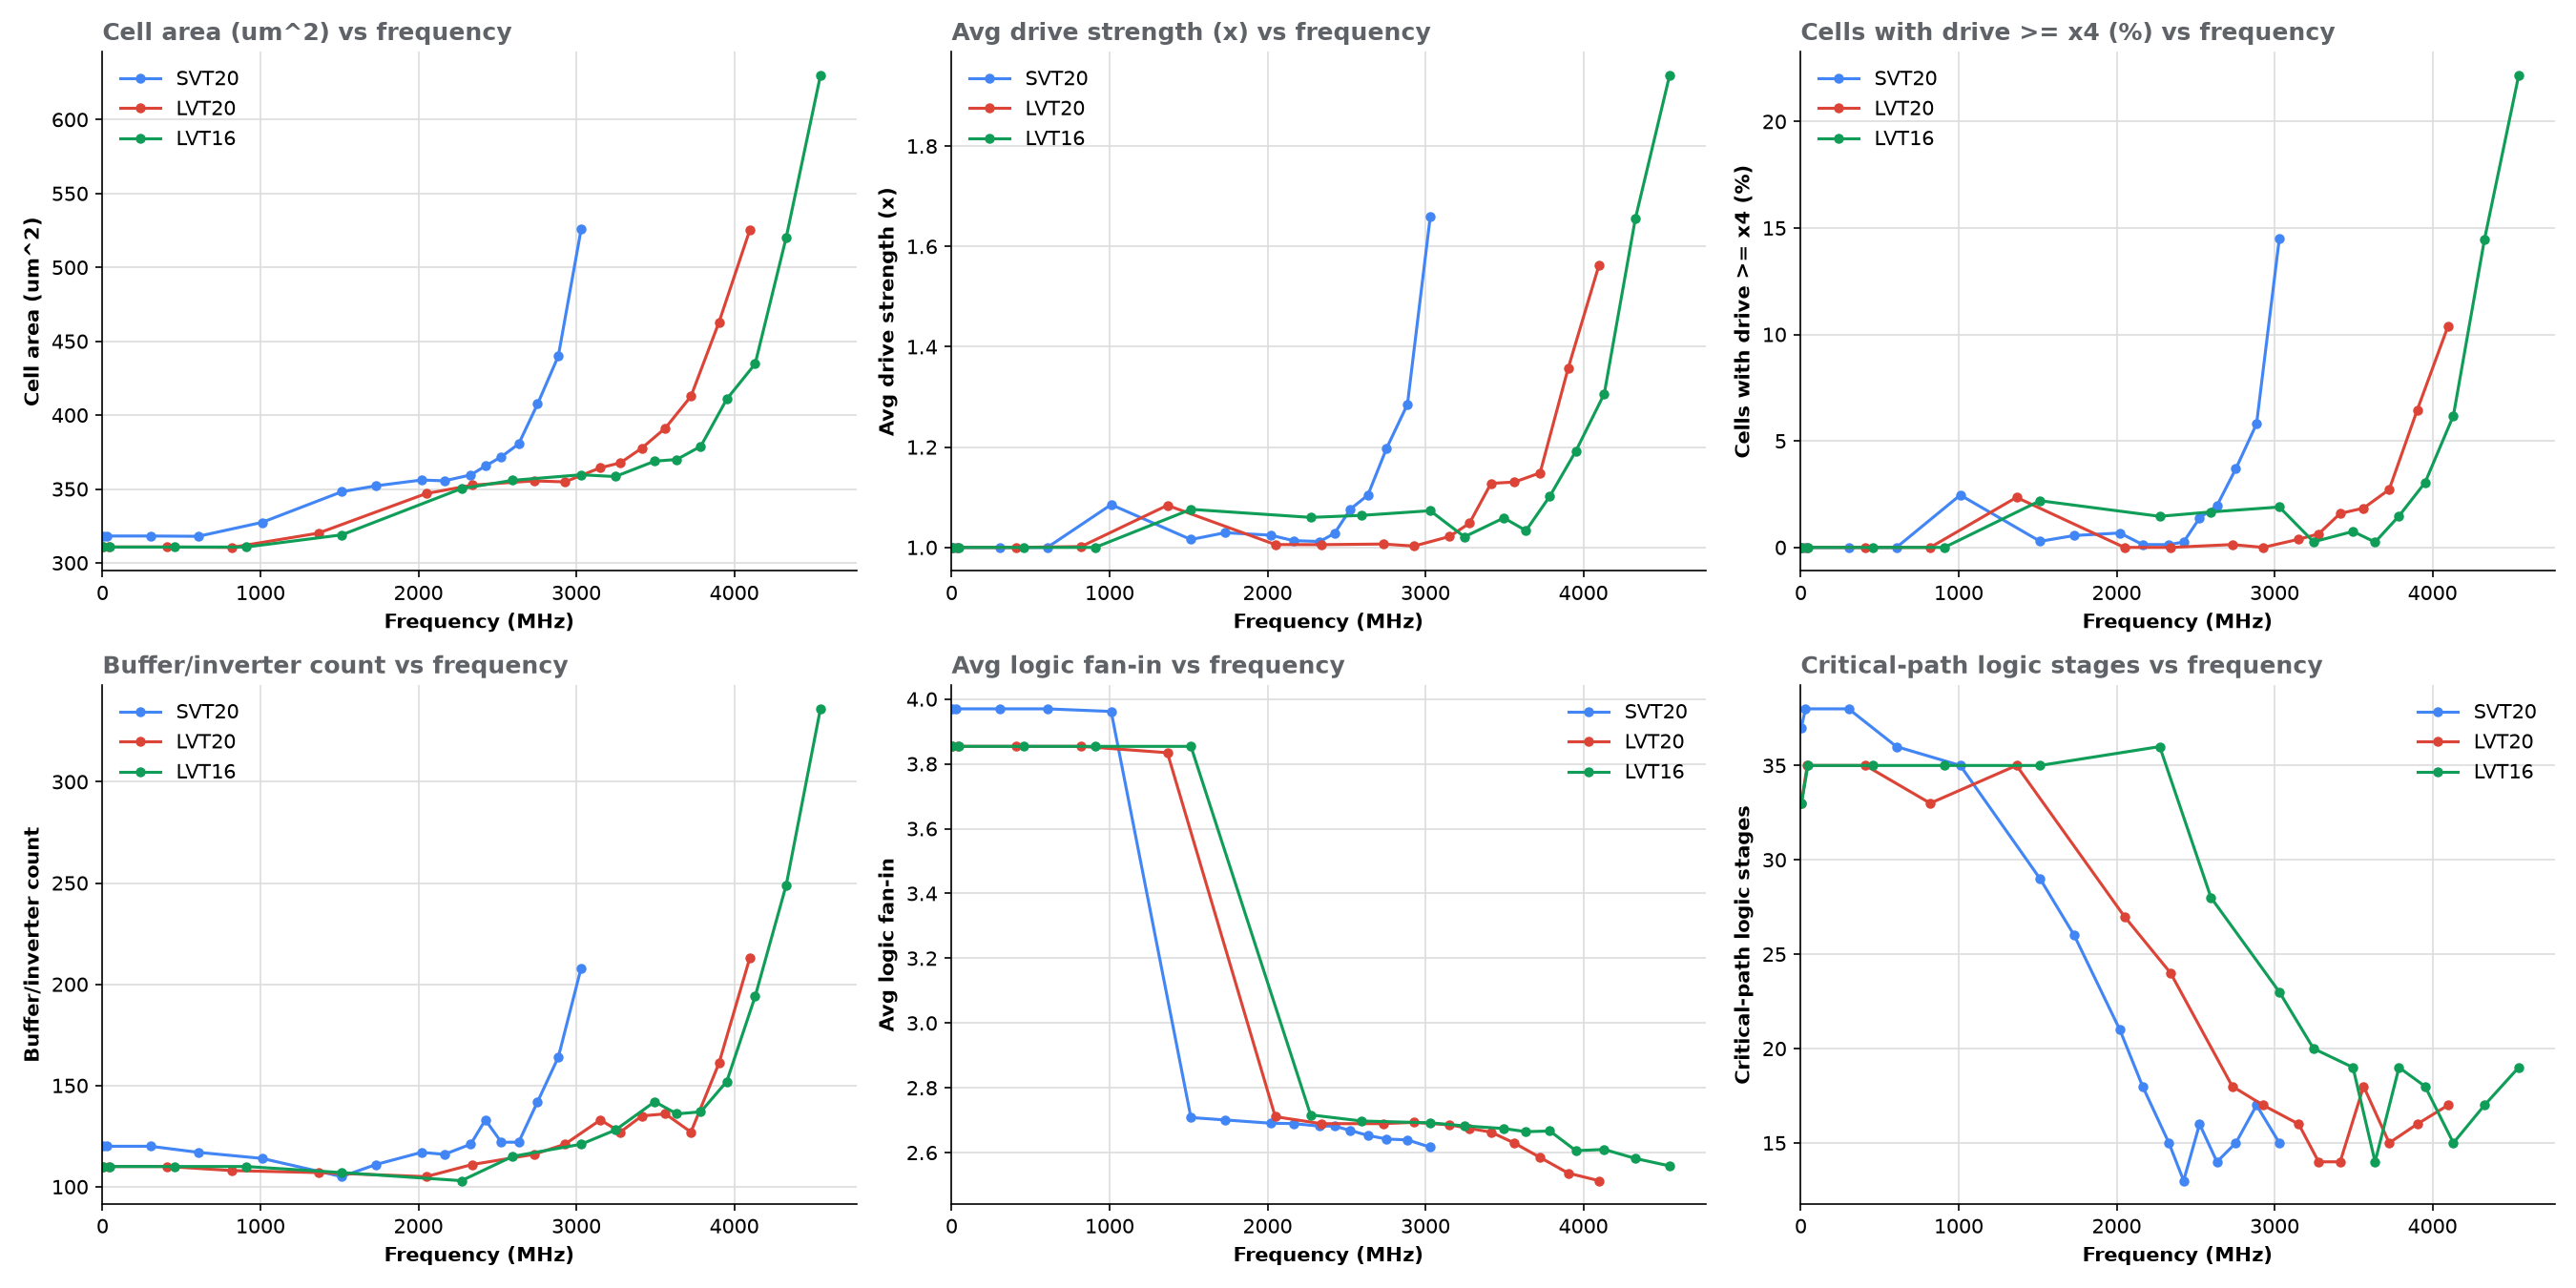
\includegraphics[width=\textwidth]{figures/ppa_vs_frequency.png}
\caption{Area, drive strength, buffer/inverter count, fan-in and critical-path length vs frequency for all three libraries.}
\label{fig:ppa}
\end{figure}

\subsection*{SVT20 (Figure~\ref{fig:energy_SVT20})}

\textbf{Performance.} At $F_{max}$ = 3030\,MHz the worst path starts at \texttt{inp\_a[5]}, ends at \texttt{prod\_reg[29]}, and passes through 15 cells with a data arrival time of 0.31\,ns (\texttt{syn\_timing.rpt}). The slack stays at 0\,ns until 606\,MHz ($5\times$), where it becomes 0.51\,ns. Below that frequency the smallest netlist DC can build is already fast enough, so its critical path (37 cells, 1.11\,ns arrival) no longer depends on the clock constraint.

\textbf{Area.} Total cell area rises from 318.2\,$\mu m^2$ at the slowest clock to 525.7\,$\mu m^2$ at $F_{max}$ (+65\%), and the cell count from 647 to 1148 (\texttt{syn\_area.rpt}). Most of the growth is near $F_{max}$: area is 348.2\,$\mu m^2$ at $2\times$ and 365.6\,$\mu m^2$ at $1.25\times$. Non-combinational area stays at 36.5\,$\mu m^2$ (32 flip-flops for \texttt{prod}), so all of the extra area is combinational logic. Buffers and inverters grow from 120 to 208 (18.8 to 44.6\,$\mu m^2$), which DC adds to drive the larger loads on the critical paths.

\textbf{Drive strength and fan-in.} From the cell list in \texttt{syn.rpt}, at the slowest clock 100\% of the combinational cells are D1 (average drive $1.00\times$). At $F_{max}$ the average drive is $1.66\times$, 14.5\% of cells are D4 or larger (29\% of combinational area), and the largest cell is D12. The cells on the critical path average $2.6\times$ drive, compared with $1.0\times$ when relaxed. The gate mix also changes: the relaxed netlist uses 139 full/half-adder cells and high-fan-in complex gates (average fan-in 3.97, 84\% with three or more inputs), while the $F_{max}$ netlist uses only 28 adder cells, 292 XOR/XNR gates and more two- and three-input AOI/OAI gates (average fan-in 2.62, 46\% with three or more inputs). Gates with fewer inputs have fewer transistors in series and lower logical effort, and the restructured logic cuts the critical path from 37 to 15 cells. The switch happens between 1010 and 1515\,MHz, where the average fan-in drops from 3.96 to 2.71 and the adder count from 139 to 119. This buys speed at the cost of more, larger cells.

\textbf{Power and energy.} Dynamic power is 2.796\,mW at $F_{max}$ and 0.0016\,mW at 3.03\,MHz, roughly proportional to frequency. Per cycle, however, $E_{Dyn}$ rises from 0.521\,pJ to 0.923\,pJ (+77\%), because the upsized, larger netlist switches more capacitance each cycle. Leakage power follows the cell area and size: 1070\,nW at $F_{max}$ and 361\,nW when relaxed. Because $E_{Leak}$ is leakage power times the clock period, it is only 0.04\% of $E_{total}$ at $F_{max}$ but 18.6\% at 3.03\,MHz. The total energy curve therefore has a minimum of 0.5226\,pJ at 303\,MHz: faster than this, upsizing raises $E_{Dyn}$; slower than this, leakage accumulates over the longer cycle.

\begin{table}[H]
\begin{center}
\small
\begin{tabular}{r|r|r|r|r|r|r|r|r|r|r|r}
\hline
f (MHz) & area & cells & buf/inv & avg drive & \% D4+ & max D & fan-in & FA/HA & XOR & path cells & arrival \\
\hline
3030 & 525.7 & 1148 & 208 & 1.66 & 14.5 & 12 & 2.62 & 28 & 292 & 15 & 0.31 \\
2424 & 365.6 & 819 & 133 & 1.03 & 0.3 & 4 & 2.68 & 117 & 174 & 13 & 0.39 \\
2020 & 356.1 & 770 & 117 & 1.02 & 0.7 & 4 & 2.69 & 117 & 174 & 21 & 0.48 \\
1515 & 348.2 & 730 & 105 & 1.02 & 0.3 & 4 & 2.71 & 119 & 173 & 29 & 0.64 \\
1010 & 327.4 & 642 & 114 & 1.09 & 2.5 & 4 & 3.96 & 139 & 1 & 35 & 0.97 \\
606 & 318.0 & 644 & 117 & 1.00 & 0.0 & 1 & 3.97 & 139 & 1 & 36 & 1.12 \\
303 & 318.2 & 647 & 120 & 1.00 & 0.0 & 1 & 3.97 & 139 & 1 & 38 & 1.12 \\
3 & 318.2 & 647 & 120 & 1.00 & 0.0 & 1 & 3.97 & 139 & 1 & 37 & 1.11 \\
\hline
\end{tabular}
\end{center}
\caption{SVT20 netlist statistics from \texttt{syn\_area.rpt}, \texttt{syn.rpt} and \texttt{syn\_timing.rpt} (area in $\mu m^2$, arrival in ns).}
\end{table}
Critical-path cells at $F_{max}$ (function\,$\times$\,drive): \texttt{XOR2x2 CKNx8 CKBx1 OAI22x1 FA1x1 XOR3x4 OAI21x2 IOA21x1 NR2x4 NR2x4 CKND2x4 INVx4 ND2x1 IAOI21x1 XOR2x1}.

\subsection*{LVT20 (Figure~\ref{fig:energy_LVT20})}

\textbf{Performance.} At $F_{max}$ = 4098\,MHz the worst path starts at \texttt{inp\_b[0]}, ends at \texttt{prod\_reg[26]}, and passes through 17 cells with a data arrival time of 0.23\,ns (\texttt{syn\_timing.rpt}). The slack stays at 0\,ns until 820\,MHz ($5\times$), where it becomes 0.38\,ns. Below that frequency the smallest netlist DC can build is already fast enough, so its critical path (33 cells, 0.82\,ns arrival) no longer depends on the clock constraint.

\textbf{Area.} Total cell area rises from 310.7\,$\mu m^2$ at the slowest clock to 525.2\,$\mu m^2$ at $F_{max}$ (+69\%), and the cell count from 628 to 1254 (\texttt{syn\_area.rpt}). Most of the growth is near $F_{max}$: area is 346.9\,$\mu m^2$ at $2\times$ and 367.7\,$\mu m^2$ at $1.25\times$. Non-combinational area stays at 36.5\,$\mu m^2$ (32 flip-flops for \texttt{prod}), so all of the extra area is combinational logic. Buffers and inverters grow from 110 to 213 (17.2 to 43.7\,$\mu m^2$), which DC adds to drive the larger loads on the critical paths.

\textbf{Drive strength and fan-in.} From the cell list in \texttt{syn.rpt}, at the slowest clock 100\% of the combinational cells are D1 (average drive $1.00\times$). At $F_{max}$ the average drive is $1.56\times$, 10.4\% of cells are D4 or larger (20\% of combinational area), and the largest cell is D12. The cells on the critical path average $2.3\times$ drive, compared with $1.0\times$ when relaxed. The gate mix also changes: the relaxed netlist uses 139 full/half-adder cells and high-fan-in complex gates (average fan-in 3.85, 89\% with three or more inputs), while the $F_{max}$ netlist uses only 17 adder cells, 372 XOR/XNR gates and more two- and three-input AOI/OAI gates (average fan-in 2.51, 37\% with three or more inputs). Gates with fewer inputs have fewer transistors in series and lower logical effort, and the restructured logic cuts the critical path from 33 to 17 cells. The switch happens between 1366 and 2049\,MHz, where the average fan-in drops from 3.83 to 2.71 and the adder count from 139 to 118. This buys speed at the cost of more, larger cells.

\textbf{Power and energy.} Dynamic power is 4.055\,mW at $F_{max}$ and 0.0023\,mW at 4.10\,MHz, roughly proportional to frequency. Per cycle, however, $E_{Dyn}$ rises from 0.558\,pJ to 0.989\,pJ (+77\%), because the upsized, larger netlist switches more capacitance each cycle. Leakage power follows the cell area and size: 13400\,nW at $F_{max}$ and 4660\,nW when relaxed. Because $E_{Leak}$ is leakage power times the clock period, it is only 0.33\% of $E_{total}$ at $F_{max}$ but 67.1\% at 4.10\,MHz. The total energy curve therefore has a minimum of 0.5699\,pJ at 410\,MHz: faster than this, upsizing raises $E_{Dyn}$; slower than this, leakage accumulates over the longer cycle.

\begin{table}[H]
\begin{center}
\small
\begin{tabular}{r|r|r|r|r|r|r|r|r|r|r|r}
\hline
f (MHz) & area & cells & buf/inv & avg drive & \% D4+ & max D & fan-in & FA/HA & XOR & path cells & arrival \\
\hline
4098 & 525.2 & 1254 & 213 & 1.56 & 10.4 & 12 & 2.51 & 17 & 372 & 17 & 0.23 \\
3279 & 367.7 & 820 & 127 & 1.05 & 0.6 & 8 & 2.67 & 116 & 176 & 14 & 0.29 \\
2732 & 355.5 & 776 & 116 & 1.01 & 0.1 & 4 & 2.69 & 115 & 178 & 18 & 0.35 \\
2049 & 346.9 & 732 & 105 & 1.01 & 0.0 & 2 & 2.71 & 118 & 174 & 27 & 0.47 \\
1366 & 320.1 & 628 & 107 & 1.08 & 2.3 & 4 & 3.83 & 139 & 1 & 35 & 0.71 \\
820 & 310.5 & 626 & 108 & 1.00 & 0.0 & 2 & 3.85 & 139 & 1 & 33 & 0.82 \\
410 & 310.7 & 628 & 110 & 1.00 & 0.0 & 1 & 3.85 & 139 & 1 & 35 & 0.82 \\
4 & 310.7 & 628 & 110 & 1.00 & 0.0 & 1 & 3.85 & 139 & 1 & 33 & 0.82 \\
\hline
\end{tabular}
\end{center}
\caption{LVT20 netlist statistics from \texttt{syn\_area.rpt}, \texttt{syn.rpt} and \texttt{syn\_timing.rpt} (area in $\mu m^2$, arrival in ns).}
\end{table}
Critical-path cells at $F_{max}$ (function\,$\times$\,drive): \texttt{CKBx1 XNR2x1 OAI22x1 XOR2x1 XOR2x2 XNR2x2 XNR2x4 ND2x1 INVx1 AOI21x1 ND2x2 AOI21x4 OAI21x8 AOI21x4 OAI21x4 AOI21x1 XOR2x1}.

\subsection*{LVT16 (Figure~\ref{fig:energy_LVT16})}

\textbf{Performance.} At $F_{max}$ = 4545\,MHz the worst path starts at \texttt{inp\_a[13]}, ends at \texttt{prod\_reg[27]}, and passes through 19 cells with a data arrival time of 0.20\,ns (\texttt{syn\_timing.rpt}). The slack stays at 0\,ns until 909\,MHz ($5\times$), where it becomes 0.36\,ns. Below that frequency the smallest netlist DC can build is already fast enough, so its critical path (33 cells, 0.73\,ns arrival) no longer depends on the clock constraint.

\textbf{Area.} Total cell area rises from 310.7\,$\mu m^2$ at the slowest clock to 629.8\,$\mu m^2$ at $F_{max}$ (+103\%), and the cell count from 628 to 1359 (\texttt{syn\_area.rpt}). Most of the growth is near $F_{max}$: area is 350.3\,$\mu m^2$ at $2\times$ and 370.0\,$\mu m^2$ at $1.25\times$. Non-combinational area stays at 36.5\,$\mu m^2$ (32 flip-flops for \texttt{prod}), so all of the extra area is combinational logic. Buffers and inverters grow from 110 to 336 (17.2 to 67.0\,$\mu m^2$), which DC adds to drive the larger loads on the critical paths.

\textbf{Drive strength and fan-in.} From the cell list in \texttt{syn.rpt}, at the slowest clock 100\% of the combinational cells are D1 (average drive $1.00\times$). At $F_{max}$ the average drive is $1.94\times$, 22.2\% of cells are D4 or larger (45\% of combinational area), and the largest cell is D16. The cells on the critical path average $3.7\times$ drive, compared with $1.0\times$ when relaxed. The gate mix also changes: the relaxed netlist uses 139 full/half-adder cells and high-fan-in complex gates (average fan-in 3.85, 89\% with three or more inputs), while the $F_{max}$ netlist uses only 18 adder cells, 302 XOR/XNR gates and more two- and three-input AOI/OAI gates (average fan-in 2.56, 38\% with three or more inputs). Gates with fewer inputs have fewer transistors in series and lower logical effort, and the restructured logic cuts the critical path from 33 to 19 cells. The switch happens between 1515 and 2273\,MHz, where the average fan-in drops from 3.85 to 2.72 and the adder count from 139 to 121. This buys speed at the cost of more, larger cells.

\textbf{Power and energy.} Dynamic power is 5.498\,mW at $F_{max}$ and 0.0025\,mW at 4.55\,MHz, roughly proportional to frequency. Per cycle, however, $E_{Dyn}$ rises from 0.547\,pJ to 1.210\,pJ (+121\%), because the upsized, larger netlist switches more capacitance each cycle. Leakage power follows the cell area and size: 43200\,nW at $F_{max}$ and 10400\,nW when relaxed. Because $E_{Leak}$ is leakage power times the clock period, it is only 0.78\% of $E_{total}$ at $F_{max}$ but 80.7\% at 4.55\,MHz. The total energy curve therefore has a minimum of 0.5662\,pJ at 909\,MHz: faster than this, upsizing raises $E_{Dyn}$; slower than this, leakage accumulates over the longer cycle.

\begin{table}[H]
\begin{center}
\small
\begin{tabular}{r|r|r|r|r|r|r|r|r|r|r|r}
\hline
f (MHz) & area & cells & buf/inv & avg drive & \% D4+ & max D & fan-in & FA/HA & XOR & path cells & arrival \\
\hline
4545 & 629.8 & 1359 & 336 & 1.94 & 22.2 & 16 & 2.56 & 18 & 302 & 19 & 0.20 \\
3636 & 370.0 & 839 & 136 & 1.03 & 0.2 & 4 & 2.66 & 113 & 180 & 14 & 0.26 \\
3030 & 359.6 & 770 & 121 & 1.07 & 1.9 & 4 & 2.69 & 117 & 174 & 23 & 0.31 \\
2273 & 350.3 & 717 & 103 & 1.06 & 1.5 & 4 & 2.72 & 121 & 170 & 36 & 0.42 \\
1515 & 319.0 & 625 & 107 & 1.08 & 2.2 & 4 & 3.85 & 139 & 1 & 35 & 0.64 \\
909 & 310.7 & 628 & 110 & 1.00 & 0.0 & 1 & 3.85 & 139 & 1 & 35 & 0.73 \\
455 & 310.7 & 628 & 110 & 1.00 & 0.0 & 1 & 3.85 & 139 & 1 & 35 & 0.73 \\
5 & 310.7 & 628 & 110 & 1.00 & 0.0 & 1 & 3.85 & 139 & 1 & 33 & 0.73 \\
\hline
\end{tabular}
\end{center}
\caption{LVT16 netlist statistics from \texttt{syn\_area.rpt}, \texttt{syn.rpt} and \texttt{syn\_timing.rpt} (area in $\mu m^2$, arrival in ns).}
\end{table}
Critical-path cells at $F_{max}$ (function\,$\times$\,drive): \texttt{CKNx2 INVx4 BUFFx4 XNR2x1 NR2x2 NR2x4 XNR2x4 XNR2x8 XOR2x8 XOR2x4 XNR2x4 ND2x2 INVx1 AOI21x4 OAI21x4 AOI21x8 OAI21x4 AOI21x1 XNR2x1}.

\subsection*{Optimal operating frequency}

\begin{center}
\small
\begin{tabular}{l|l|l|l}
\hline
Library & (a) Area-constrained & (b) Timing-critical & (c) Energy-constrained \\
\hline
SVT20 & 606 MHz (318.0 $\mu m^2$) & 3030 MHz (525.7 $\mu m^2$) & 303 MHz (0.5226 pJ) \\
LVT20 & 820 MHz (310.5 $\mu m^2$) & 4098 MHz (525.2 $\mu m^2$) & 410 MHz (0.5699 pJ) \\
LVT16 & 909 MHz (310.7 $\mu m^2$) & 4545 MHz (629.8 $\mu m^2$) & 909 MHz (0.5662 pJ) \\
\hline
\end{tabular}
\end{center}
\textbf{SVT20.} (a) For an area-constrained design I would run at 606\,MHz (1.65\,ns). This is the fastest point whose area is within 1\% of the minimum (318.0\,$\mu m^2$); a slower clock gives no further area savings, only lower throughput. (b) For a timing-critical design I would run at $F_{max}$ = 3030\,MHz, which costs 65\% more area and 77\% more energy per cycle than the minimum. (c) For an energy-constrained design I would run at 303\,MHz (3.3\,ns), the minimum of $E_{total}$ (0.5226\,pJ/cycle); since 606\,MHz is within 2\% of this energy (0.5237\,pJ), it is also a good choice with higher throughput.

\textbf{LVT20.} (a) For an area-constrained design I would run at 820\,MHz (1.22\,ns). This is the fastest point whose area is within 1\% of the minimum (310.5\,$\mu m^2$); a slower clock gives no further area savings, only lower throughput. (b) For a timing-critical design I would run at $F_{max}$ = 4098\,MHz, which costs 69\% more area and 74\% more energy per cycle than the minimum. (c) For an energy-constrained design I would run at 410\,MHz (2.44\,ns), the minimum of $E_{total}$ (0.5699\,pJ/cycle); since 820\,MHz is within 2\% of this energy (0.5706\,pJ), it is also a good choice with higher throughput.

\textbf{LVT16.} (a) For an area-constrained design I would run at 909\,MHz (1.1\,ns). This is the fastest point whose area is within 1\% of the minimum (310.7\,$\mu m^2$); a slower clock gives no further area savings, only lower throughput. (b) For a timing-critical design I would run at $F_{max}$ = 4545\,MHz, which costs 103\% more area and 115\% more energy per cycle than the minimum. (c) For an energy-constrained design I would run at 909\,MHz (1.1\,ns), the minimum of $E_{total}$ (0.5662\,pJ/cycle).

\textbf{Across libraries.} LVT16 reaches the highest $F_{max}$ (4545\,MHz), so it is the choice for a timing-critical design. SVT20 has the lowest minimum energy (0.5226\,pJ/cycle) because its leakage is much lower (SVT20: 1070\,nW, LVT20: 13400\,nW, LVT16: 43200\,nW at $F_{max}$), so it is the choice for an energy-constrained design. The minimum areas are close (SVT20: 318.0, LVT20: 310.5, LVT16: 310.7\,$\mu m^2$), with LVT20 the smallest. At the slowest clock, where the LVT16 and LVT20 netlists have almost the same area (310.7 and 310.7\,$\mu m^2$), LVT16 leaks 10400\,nW versus 4660\,nW, so the BWP16 cells leak 2.2$\times$ more than the BWP20 cells of the same $V_t$ in exchange for their higher speed. Low-$V_t$ cells switch faster but leak more, which is why the LVT libraries have higher $F_{max}$ and a steeper rise in total energy at low frequency.

\end{document}
